\begin{center}
  \Large
  \textbf{BIOGRAFI PENULIS}
\end{center}

\addcontentsline{toc}{chapter}{BIOGRAFI PENULIS}

\vspace{2ex}

\begin{wrapfigure}{L}{0.3\textwidth}
  \centering
  \vspace{-3ex}
  % Ubah file gambar berikut dengan file foto dari mahasiswa
  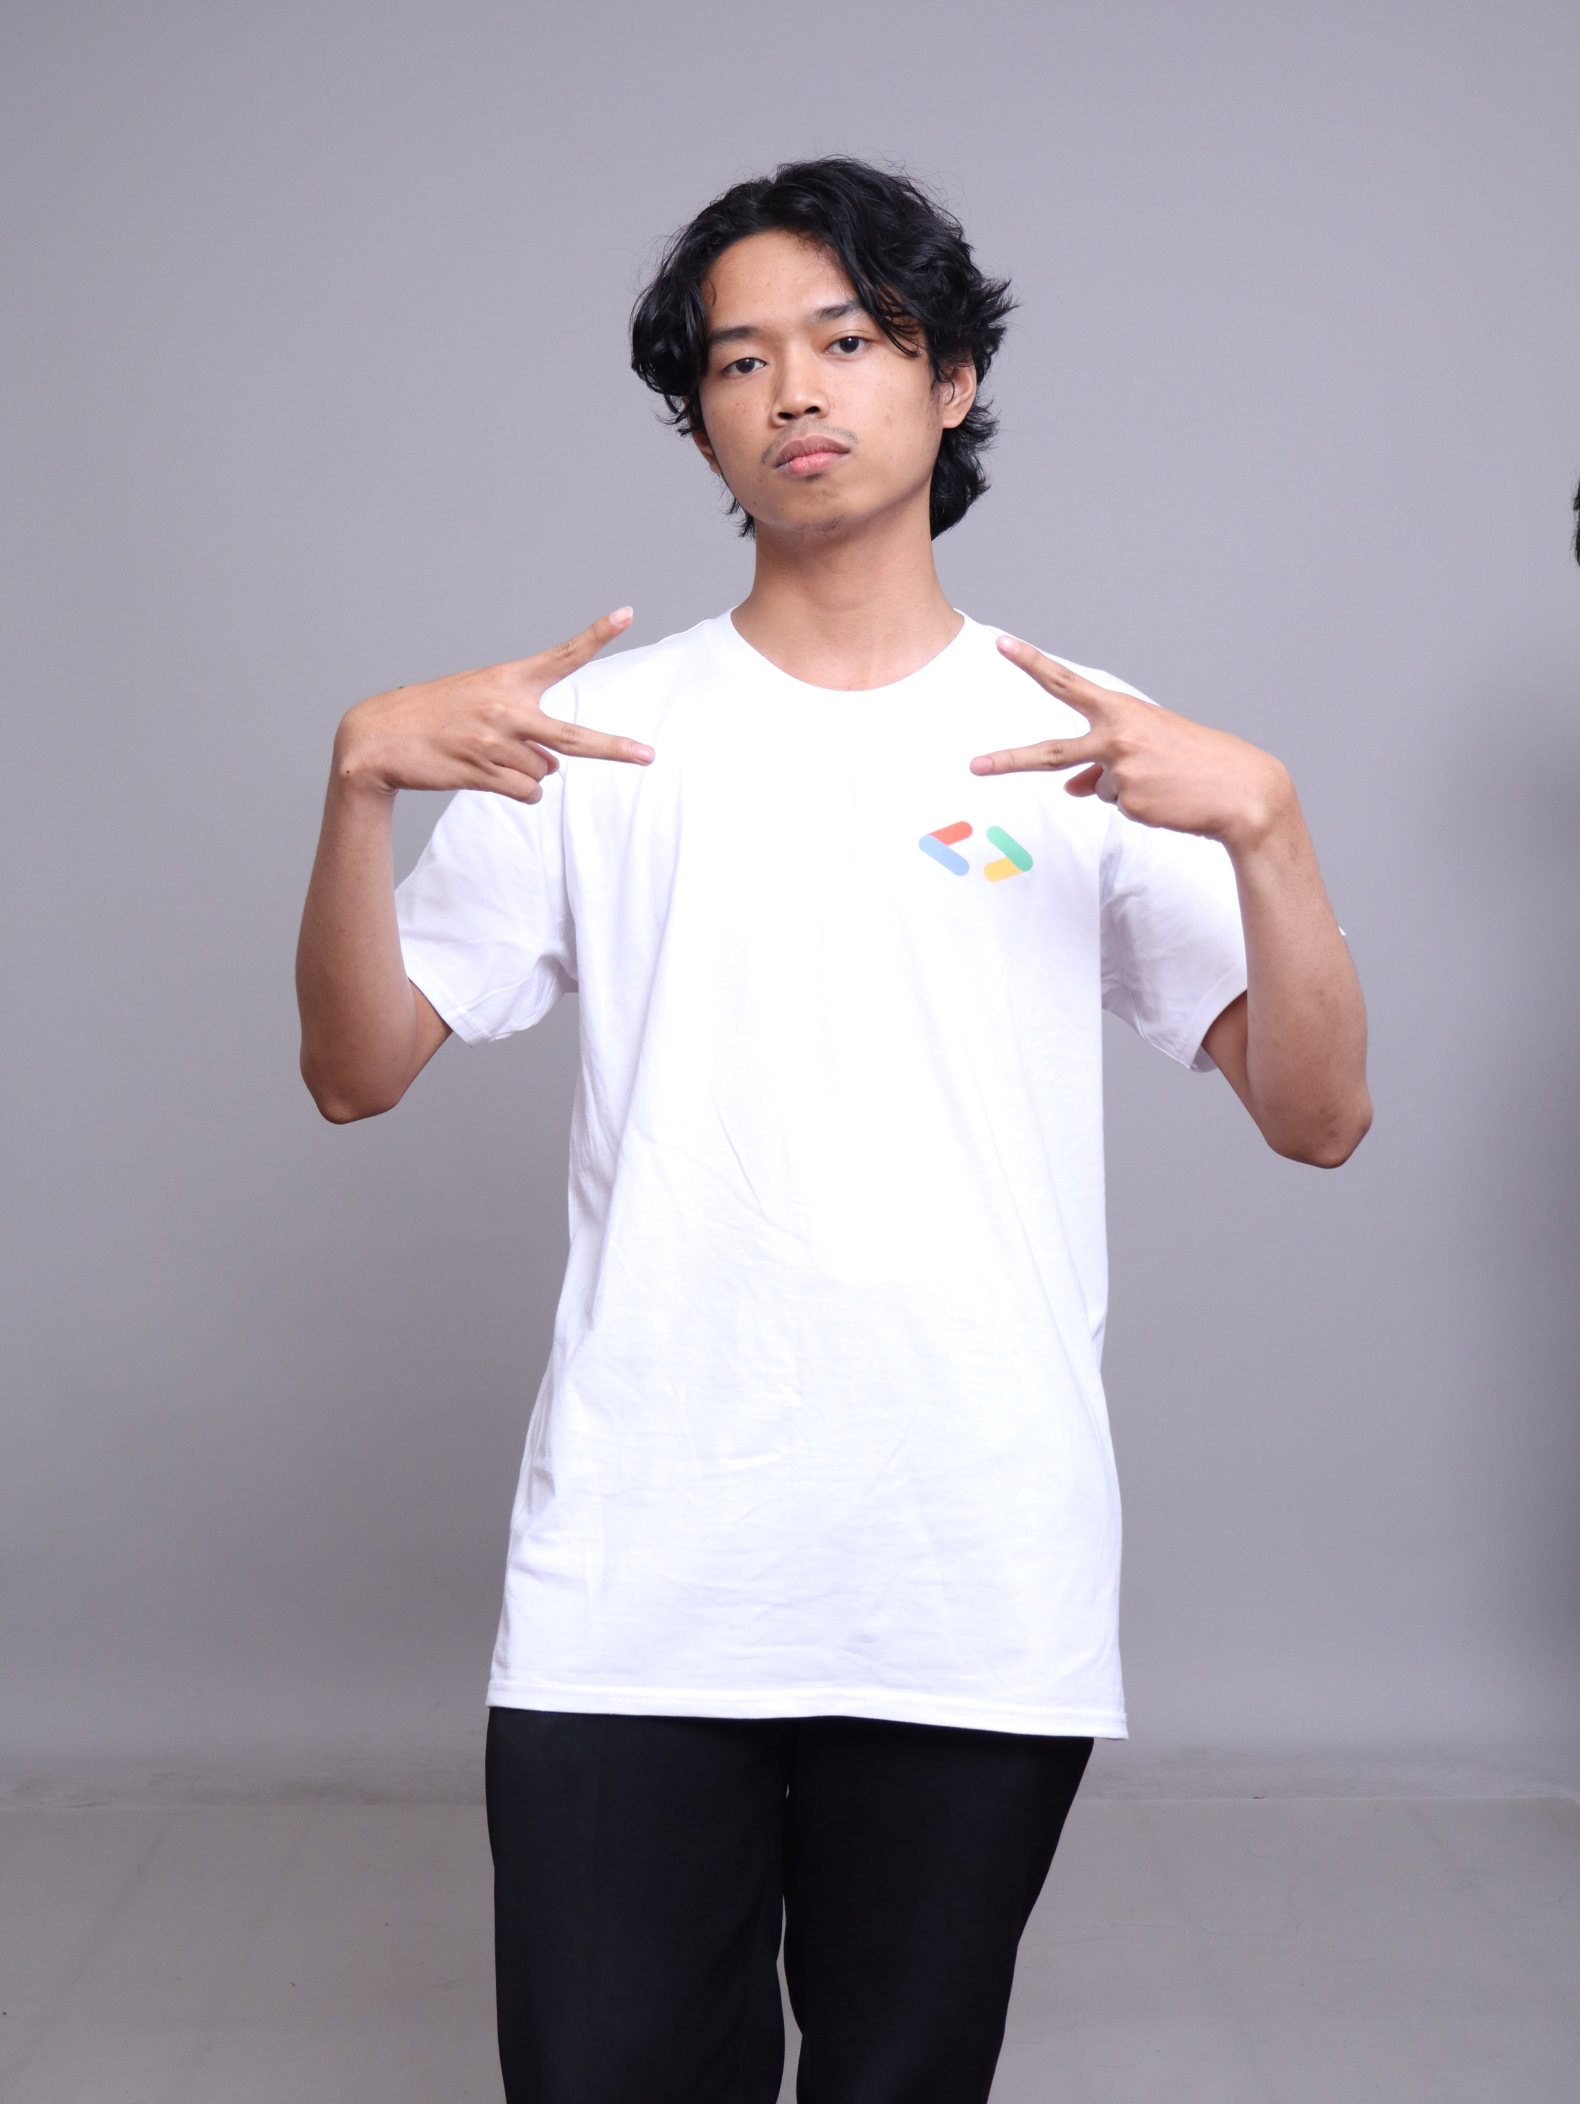
\includegraphics[width=0.3\textwidth]{gambar/Ariq 2.png}
  \vspace{-4ex}
\end{wrapfigure}

% Ubah kalimat berikut dengan biografi dari mahasiswa
\name{}, lahir pada 29 Oktober 2003 satu hari setelah hari sumpah pemuda. Sampai pada saat teks ini dituliskan, dia adalah seorang laki-laki yang baru berumur 21 tahun dengan asal dari Bangkalan, Madura. Merupakan salah satu anak dari pasangan suami istri, Moh. Rasyid dan Nurul Mualifah. Dia memiliki 6 saudara kandung dengan 2 kakak perempuan, 2 adik laki-laki, dan 2 adik perempuan. Riki, adalah panggilan rumahnya, dimana ia dibesarkan di desa Batah Barat, kec. Kwanyar. dia adalah anak yang nakal dan sering bertengkar dengan kedua kakak perempuannya\dots

Maulana Tazakka, dia mulai mengenyam pendidikan di TK 2 Batah Timur selama 6 bulan, dilanjutkan dengan sekolah di SDN 2 Batah Barat, disana dia adalah orang yang cengeng namun aktif dalam olimpiade tingkat kabupaten. Di jenjang berikutnya, dia masuk di SMPN 1 Kwanyar, di sekolah ini dia berhasil menembus dan lolos ke olimpiade tingkat Nasional pada bidang Matematika di ajang OSN. Dia lanjut mengenyam pendidikan di sekolah beda kota dimana dia masuk asrama. SMAN 3 Pamekasan adalah tujuannya, selama 3 tahun ia baru pertama kali lolos dalam ajang nasional dalam olimpiade Primagama Mencari Juara tingkat nasional dan meraih peringkat 5. Selebihnya, dia selalu gagal. Di jenjang sma, dia mulai belajar menyatakan perasaannya pada lawan jenisnya\dots

Ada satu hal yang menarik terkait pertemanannya. Di setiap tingkat, dia hanya memiliki satu teman yang paling dekat. Di jenjang SD, dia dekat dengan seorang anak bernama Ulum meskipun dia tahu dia sedang dimanfaatkan oleh dia dan temannya. Di jenjang SMP, dia dekat dengan seorang anak bernama Eko Pratama, seorangan anak dari padepokan PSHT yang memiliki karakter menyenangkan untuk diajak berbicara dan bermain bola bersama. Di jenjang SMA, ada seorang anak bernama fuad amiren yang sudah seperti kembarannya kata banyak orang di sekolah, iren sering memanggilku "ariqusu" yang merupakan representasi jepang dari nama ariq\dots

Saat ini, dia adalah mahasiswa semester 7 di Teknik Komputer ITS, dimana dia mempelajari banyak hal berkaitan dengan teknologi mulai dari pembuatan web, perangkat IoT, dan konsep Robotika. Dia mendalami bidang pembuatan aplikasi dan game dengan framework yang biasa dia gunakan adalah flutter dan firebase untuk app development serta unity gae engine untuk game development. Dia juga cukup piawai dalam pembuatan model artificial Intelligent dengan framework keras tensorflow dan juga pytorch. Kuliah merupakan masa paling berarti bagi perkembangannya sebagai individu dan karir, satu kegagalan setelah kegagalan yang lainnya hingga mengantarkannya ke satu keberhasilan yang memuaskan. Menekuni dunia IT tidaklah mudah, begitu banyak hal yang perlu dipelajari, begitu banyak waktu yang perlu dikorbankan, kolaborasi dan kerjasama dengan orang lain untuk menyelesaikan berbagai macam proyek yang diberikan\dots

Di masa depan dia bercita cita untuk memajukan standar hidup masyarakat Indonesia. Ingin memiliki komunitas coding untuk kampung halamannya demi indonesia yang lebih melek teknologi. Jika pada akhirnya bekerja, dia ingin menjadi Software atau AI Engineer, dimana dia dapat mengimplementasikan pengetahuannya untuk menyelesaikan permasalahan publik, sistem sistem rumit dan kemajuan negeri ini sendiri. Ariq memiliki karakter Ekstrovert namun hanya aktif ketika bersama dengan teman dekatnya saja. Dia memiliki masalah susah fokus dalam satu pekerjaan, yang selalu menjadi penyebab dia gagal meniti karir selama ini. Dia memiliki \emph{mindset} untuk selalu berkembang, kreativitasnya dalam menyelesaikan masalah tak perlu diragukan, dan skill problem solving yang pastinya dia miliki. Dia juga peka terhadap permasalahan sekitarnya, namun siapalah dia yang tak berdaya dihadapan sistem yang telah lama ada.